\chapter{Proposed Work}
\label{ch:proposed}


\section{Chapter Introduction}
Armed with insights from the negative results of the annotation experiments that discourse structures cannot be learned in an unsupervised fashion while annotating discourse is a subjective and ambiguous task, my proposed work addresses three pieces missing from most existing discourse theories. First, discourse judgements are not solely from the point of view of the writer, but also of the reader. Second, the reader is biased, and their beliefs influence how they interpret the discourse of a text. Third, a given text can have multiple, valid discourse labels, depending on the reader.\footnote{PDTB allows for multiple labels, but was used as a last resort when annotators could not agree \citep{Versley:2011}.} These aspects are captured well in the theoretical work of \citet{Asher:2018} that frames conversations as a game of exchanging messages, where the reader is a judge of the game's success. I propose to create a new dataset that allows for multiple labels on a single item, and new tasks for predicting these labels first using text alone, and then using information from the judges (the annotators). Because ambiguity and subjectivity are both more prevalent and easier to identify in dialogue vs. monologue and the taxonomies of discourse relations are onerous for a crowd-sourced worker to learn, I focus my dataset on \emph{conversations} that are labeled with \emph{dialogue acts}. Dialogue acts, loosely defined as speech acts in dialogue, describe the performative actions in an utterance (e.g., requesting for help or thanking).

\section{Background}
I present an overivew of ambiguity in discourse and how conversations are treated as games.

\subsection{Discourse Ambiguity} Several works have recognized the inherent ambiguity of discourse, ranging from coreference resolution to the rhetorical structures in the three major discourse frameworks of RST, SDRT, and PDTB \citep{Poesio:2019,Das:2017,Asher:2003,Versley:2011}. These works have found the ambiguities stem from multiple, valid interpretations and are not the result of bad annotation. \citet{Poesio:2019} create a corpus of crowd-sourced coreferences and show there is often inherent ambiguity in resolving an anaphoric mention. In PDTB, discourse connectives are annotated for senses and discourse relations are annotated between two arguments. While PDTB allows for multiple senses for discourse connectives, only 5.5\% have more than one sense as it was effectively used as a last resort when annotators could not agree \cite{Versley:2011}.\footnote{These numbers are for PDTB 2.0. Interestingly, the PDTB 3.0 annotation manual adds an additional case for allowing multiple labels for discourse relations.} \citet{Versley:2011} points to the value of having ambiguous connectives that are helpful in identifying when more than one discourse relation can hold. In RST, most ambiguities arise during the relation-labeling task, and particularly for the higher-level nodes that attempt to encompass larger spans of text \cite{Das:2017}. 

To handle this ambiguity, many propose underspecified structures that leave the ambiguous part of the discourse unresolved. However, \citet{Webber:2012} argues that variability in the annotation of PDTB relations is not caused by genuine ambiguities, but instead is a result of a lack of deeper understanding of how to comprehensively annotate discourse. While I agree some discrepancies could be resolved by better annotation, I nevertheless believe a single text can be interpreted to have multiple valid discourse structures. 

\subsection{Conversation as a game} In \citet{Asher:2018}, conversations are presented as message exchange games.\footnote{I cite this as the main work that most elaborates on the theory. Other works by the authors describing different parts of the theory include \citet{Asher:2016,Asher:2017}.} The players (or conversants) each have their own conversational goal, while a third party, the judge, evaluates the success, which is defined as achieving that goal. Importantly, the judge is biased: different judges can have different interpretations of the same text, depending on their beliefs and personal preferences. As the conversation progresses, each turn in the conversation is evaluated by the judge and contributes to alternate histories of the entire conversation. This framework can be extended beyond dialogue and applied to more expository text where there is only one player. In this work, I focus on question-answer dialogues where I believe ambiguity is more prevalent and easier to annotate. 
%In future work, I would explore other genres as \cite{Das:2017}  Even on less controversial texts like news reports, agreement by expert RST annotators is fairly low— Das et al. 2017

\section{Short Term}
In the short term, I focus on the ambiguity of discourse. I propose to create a dataset of question-answer pairs extracted from U.S. Congressional hearings. Each question-answer is labeled with \emph{multiple}, valid dialog acts and a question type. I design a model to predict the question-answer label set, and propose variants of this model that additionally condition on the context of previous question-answers or the question type.

\subsection{Dataset: Q\&A in Congressional Hearings}
A first step in operationalizing the key parts of conversations-as-games theory is to find an appropriate dataset. The desiderata for the data are: (i) must contain controversy identifiable by a crowd-sourced worker, (ii) documents must contain a strong signal of ambiguity (more than 1/10 of the statements must be ambiguous), (iii) the data must be plentiful enough for use in a neural network model (more than 1,000 documents). Transcripts of congressional hearings, in particular the question-answer portions, fit these requirements: (i) most hearings are politically polarized, (ii) a preliminary analysis of two transcripts shows sufficient ambiguity (60\% and 12\%, respectively), (iii) over 5,000 transcripts exist in 2018-2019 alone.

\begin{table}[t]
    \centering
    \begin{tabular}{p{11cm}}
    \toprule
    \textit{Mr. Engel:} So do you adjust your algorithms to prevent individuals interested in violence or nefarious activities from being connected with other like-minded individuals?

\textit{Mr. Zuckerberg:} \textbf{Sorry. Could you repeat that?} \texttt{request for information} or \texttt{stall}

\textit{Mr. Engel:} Do you adjust your algorithms to prevent individuals interested in violence or bad activities from being connected with other like-minded individuals?

\textit{Mr. Zuckerberg:} \textbf{Congressman, yes. That is certainly an important thing that we need to do.} \texttt{acknowledge} or \texttt{answer}\\
\midrule
\textit{Mr. Levin:} [...] The agenda, and I have known people from the EPA in past administrations, both Republican and Democratic--their agenda, at least their original agenda as intended from President Nixon and both the Democrats and Republicans who supported the Clean Air Act and the Clean Water Act at the time, was simply to protect human health and the environment.    On the other hand, Dr. Dayaratna, I find your agenda perhaps a bit more suspect. So, please answer yes or no, just yes or no. Do studies \underline{funded by fossil fuel money} have an agenda?

\textit{Dr. Dayaratna:} \textbf{I am sorry, Congressman. I cannot answer that question because that has nothing to do with my research, so---}\\
    \bottomrule
    \end{tabular}
    \caption{Top: examples of answers (bold) that could have multiple interpretations. Bottom: example of a ``loaded'' question with a presupposition (underlined), which is not accepted by the respondent and results in a non-answer (bold).}
    \label{tab:example}
\end{table}

\begin{table}[t]
    \centering
    \begin{tabular}{p{11cm}}
    \toprule
1. So you have mentioned several times that you started Facebook in your dorm room, 2004. 15 years, 2 billion users and \textbf{several, unfortunately, breaches of trust later}, is Facebook today the same kind of company you started with a Harvard.edu email address?\\
2. Why wasn't explaining what Facebook does with users' data \textbf{higher} priority for you as a cofounder and now as CEO? \\
3. Yes or no, is Facebook changing any user default settings to be \textbf{more} privacy protective? \\
4. Will you make the commitment to change all the user--to changing all the user default settings to minimize to the greatest extent possible the collection and use of users' data? \textbf{I don't think that is hard for you to say yes to, unless I am missing something.}\\
5. How can consumers have control over their data \textbf{when Facebook doesn't have control over the data itself}?\\
    \bottomrule
    \end{tabular}
    \caption{Examples of ``loaded" questions with the loaded part in bold.}
    \label{tab:example_loaded}
\end{table}

Table \ref{tab:example} contains excerpts from two separate congressional hearings. The first example illustrates how responses to questions are sometimes ambiguous (here analyzed as speech acts): Zuckerberg's first response could be interpreted as either a \emph{request for information} if you believe he is being sincere, or as \emph{stalling} for time if you believe he is being evasive. His second response can be interpreted either as an \emph{acknowledgement} that Zuckerberg has now understood the question, or as an actual (affirmative) \emph{answer} to Engel's question about adjusting the algorithms. The second example illustrates how the questions themselves often have politically-charged presuppositions, which cannot be answered in a straightforward manner if the respondent wishes to reject the presupposition. These questions often lead to indirect or even non-answers, thus directly influencing the interpretation of valid dialog act labels. I describe these types of questions as ``loaded'' and as illustrated in the examples of Table \ref{tab:example_loaded} can also include implicatures and other linguistic devices. 

\subsection{New taxonomy for subjective discourse}
Existing taxonomies of discourse relations abound, including RST, PDTB, SDRT, and even those within RST are further modified depending on the corpus. However, we argue here that none of these taxonomies will suit our purpose of allowing untrained annotators to label ambiguities in dialogues.

In \cite{Asher:2018}, the authors work through an example of discourse ambiguity using underspecified logical forms in SDRT. Similar to the congressional hearings, the ambiguity stems from a controversial questioning, in this case between a reporter (Rachel) and a spokesperson for a Senator:

\begin{enumerate}
\item \label{ex:1}
\begin{enumerate}
\setlength\itemsep{0em}
 \item Reporter: On a different subject is there a reason that the Senator won’t say whether or not someone else bought some suits for him? \label{ex:1a}
\item Spokesperson: Rachel, the Senator has reported every gift he has ever received. \label{ex:1b}
\end{enumerate}
\end{enumerate}

They posit two judges: one who assumes the spokesperson is honest and the other dishonest. In the case of an honest spokesperson, their utterance in \ref{ex:1b} is interpreted as an indirect answer with the SDRT relation of \emph{Indirect Question Answer Pair}. If they are dishonest, their utterance is interpreted as non-cooperative, with the SDRT relation of \emph{Background} (where \ref{ex:1a} ``provides information about the surrounding state of affair'' in which \ref{ex:1b} occurred). It is less clear why this particular relation type is chosen, and requires a level of familiarity with SDRT that could not be achieved with crowd-sourced workers. It is clear that the distinction rests on whether the spokesperson is providing an answer (albeit indirect) or a non-answer. This type of judgement is much easier for a minimally-trained annotator to make. I therefore propose a much simpler taxonomy of labels, based on whether the question was answered, whether the answer was direct, and a subset of speech acts derived from the ISO 24617-2 standard, which builds upon annotation schemes used in well-known dialogue resources such as the SwitchBoard Corpus and DAMSL \citep{Bunt:2018}. Because questions heavily influence the type of answer, I also plan to annotate tye type of question to understand whether they are ``loaded'', for example by containing presuppositions or implicatures. 

%(and in turn, the answer is labeled with whether it is accepting or rejecting a presupposition).

When deciding upon an exact taxonomy of labels for questions and answers, I plan to annotate a small number of question-answer pairs from randomly selected congressional hearings to ensure a representative sample, followed by a test-annotation phase. 

\subsection{Crowd-sourcing Phase 1.}
I divide the crowd-sourcing tasks into two phases (Phase 2 is discussed in the long-term work Section \ref{subsec:phase2}). The goal of Phase 1 is to both validate the tasks and confirm my assumptions before collecting more data. This first phase consists of two labeling tasks: first, an annotator is asked to select all valid dialog act labels for a given question-answer; second, the annotator is asked to choose one label to categorize the question. Arriving at multiple ground-truth labels is at odds with the typical single-label approach, and I anticipate this goal will be particularly problematic when gathering annotations from crowd-sourced workers. Common strategies for selecting high-quality workers such as weeding out those with lower agreement scores will not work as I expect (and want) disagreement. I will rely on work in \citet{Dumitrache:2018} to address these issues.

\subsection{Experiment 1: Multi-label discourse} 
I design a series of experiments that increase in complexity and build upon the assumptions of previous ones. In this first experiment, I exclusively focus on modeling discourse with multiple ground truths. The task is to predict all the valid labels for a given question-answer pair. I then propose more complex models that take into account context (i.e., labels of previous question-answer pairs) and the question type, on the intuition that these are correlated and predictive of the following set of labels. I here describe my proposed models.

\begin{figure}
\RawFloats
\centering
\begin{minipage}{.5\textwidth}
  \centering
  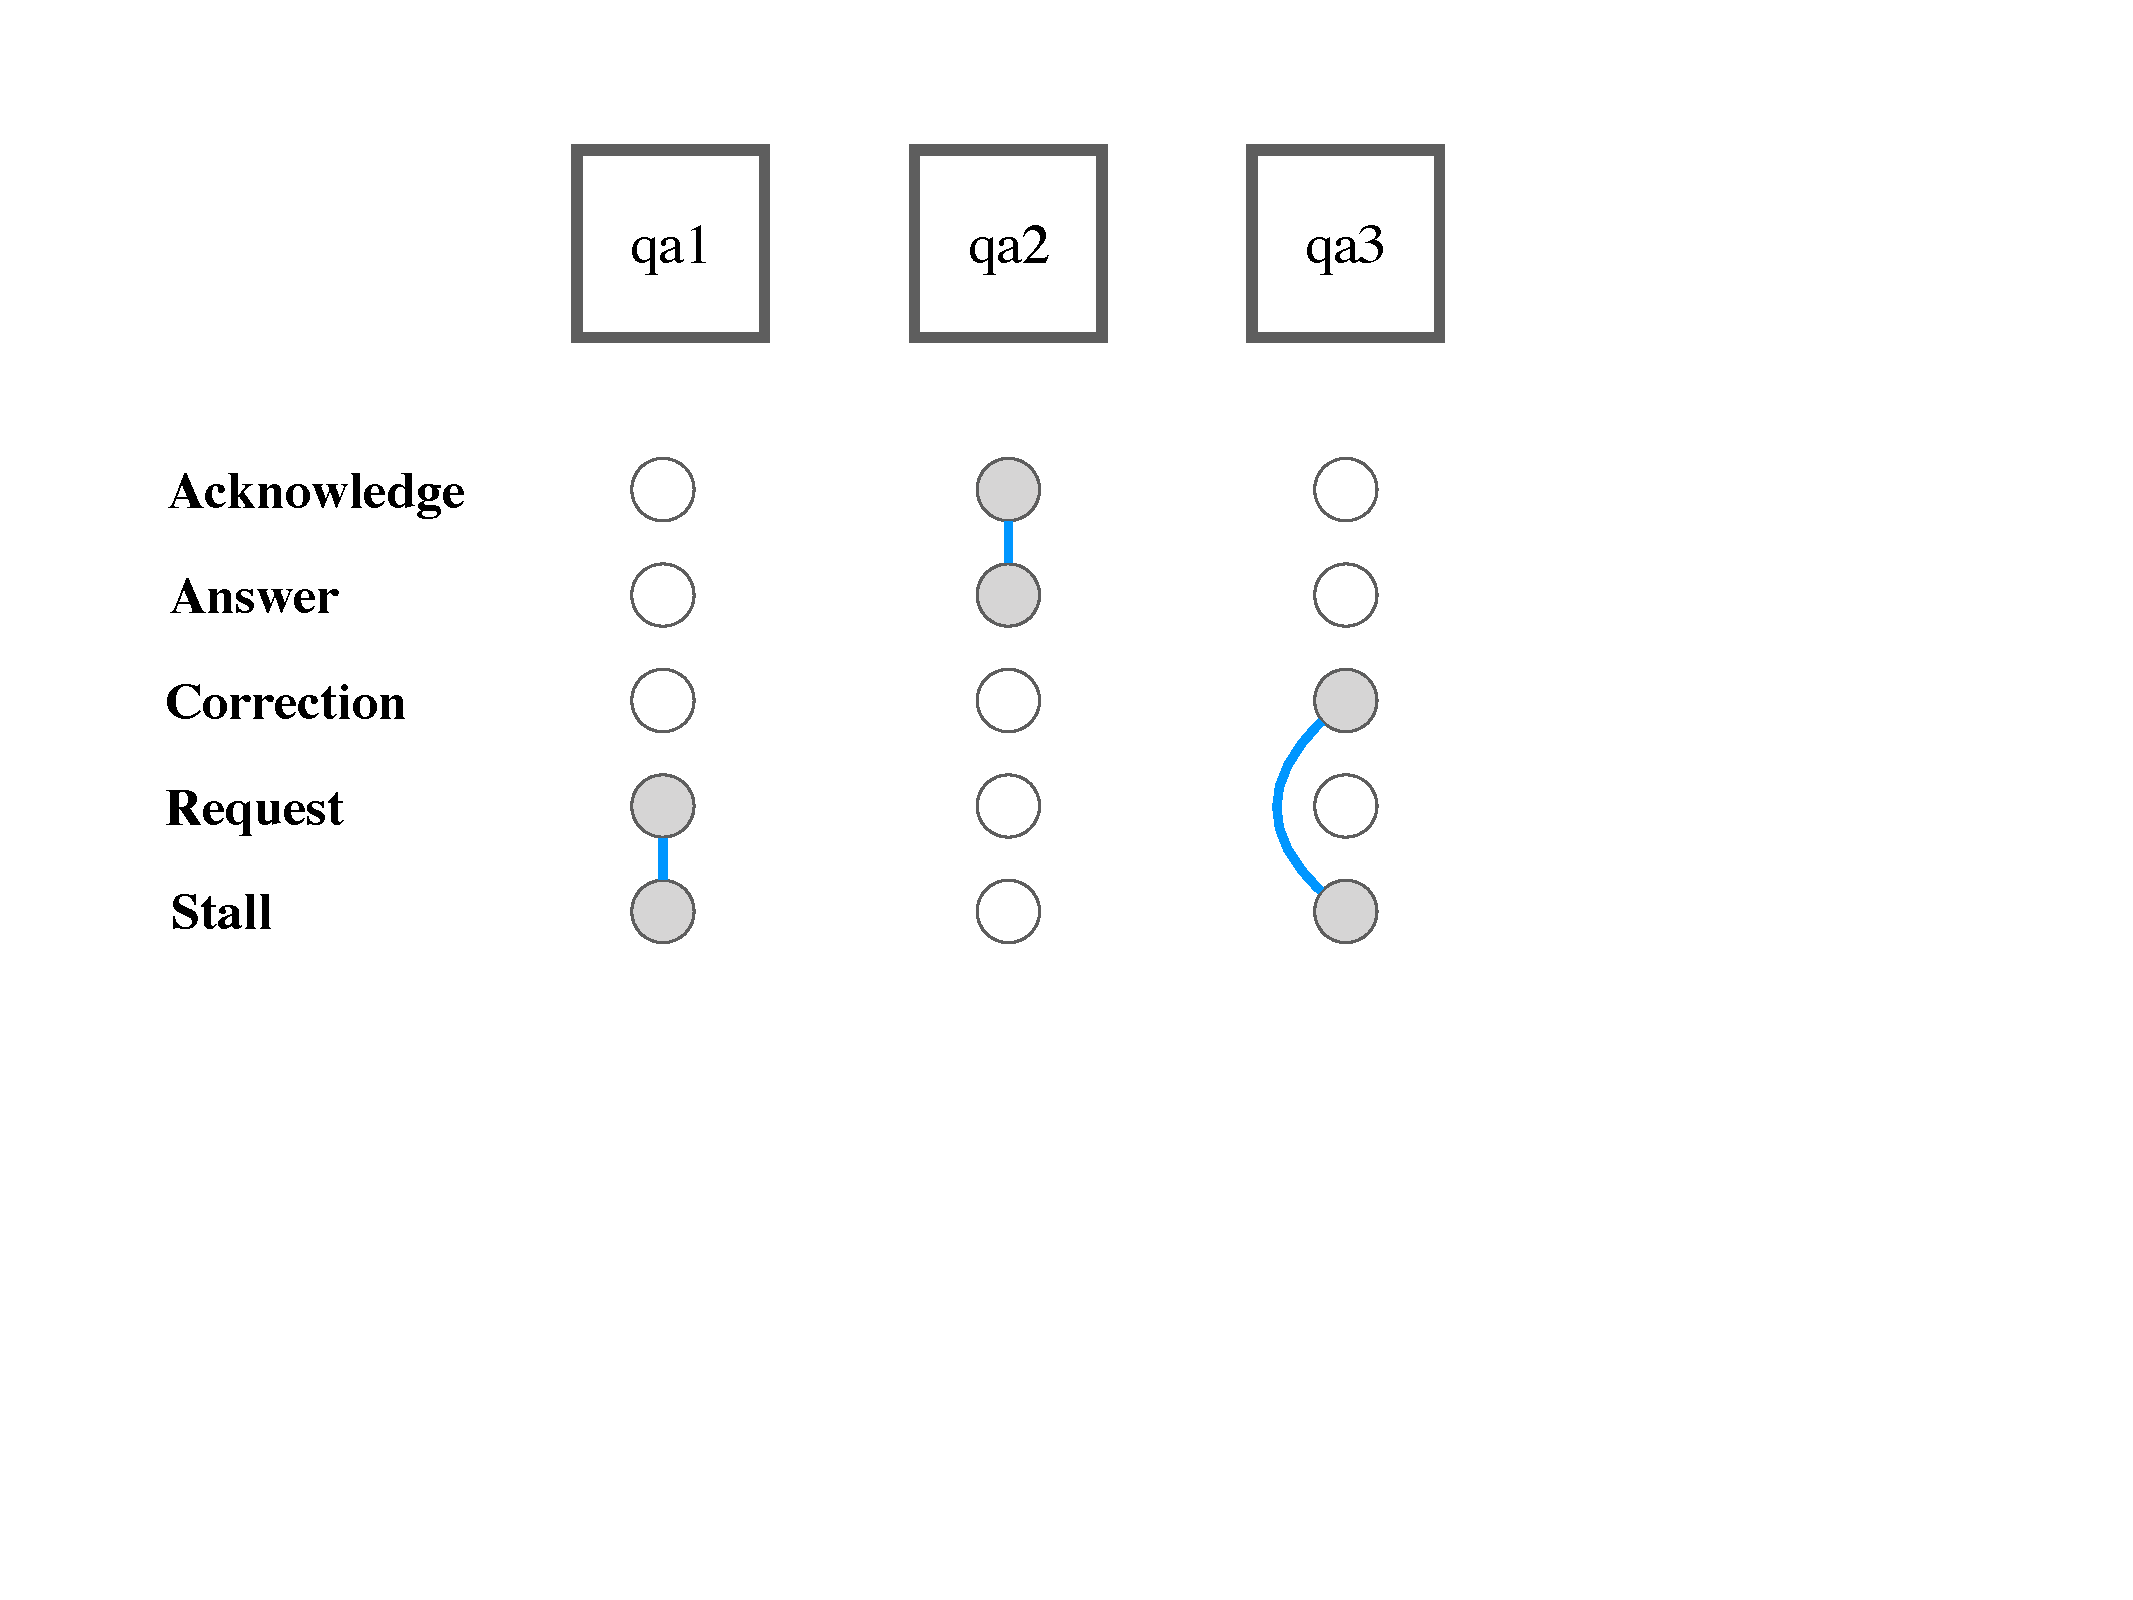
\includegraphics[width=1\linewidth]{plots/multilabel.pdf}
  \captionof{figure}{\textsc{Multi-label}: predict the set of dialog acts for a question-answer pair (qa), while modeling correlations within a set (blue).}
  \label{fig:multilabel}
\end{minipage}%
\hspace*{1.4em}
\begin{minipage}{.5\textwidth}
  \centering
  \vspace{1.3em}
  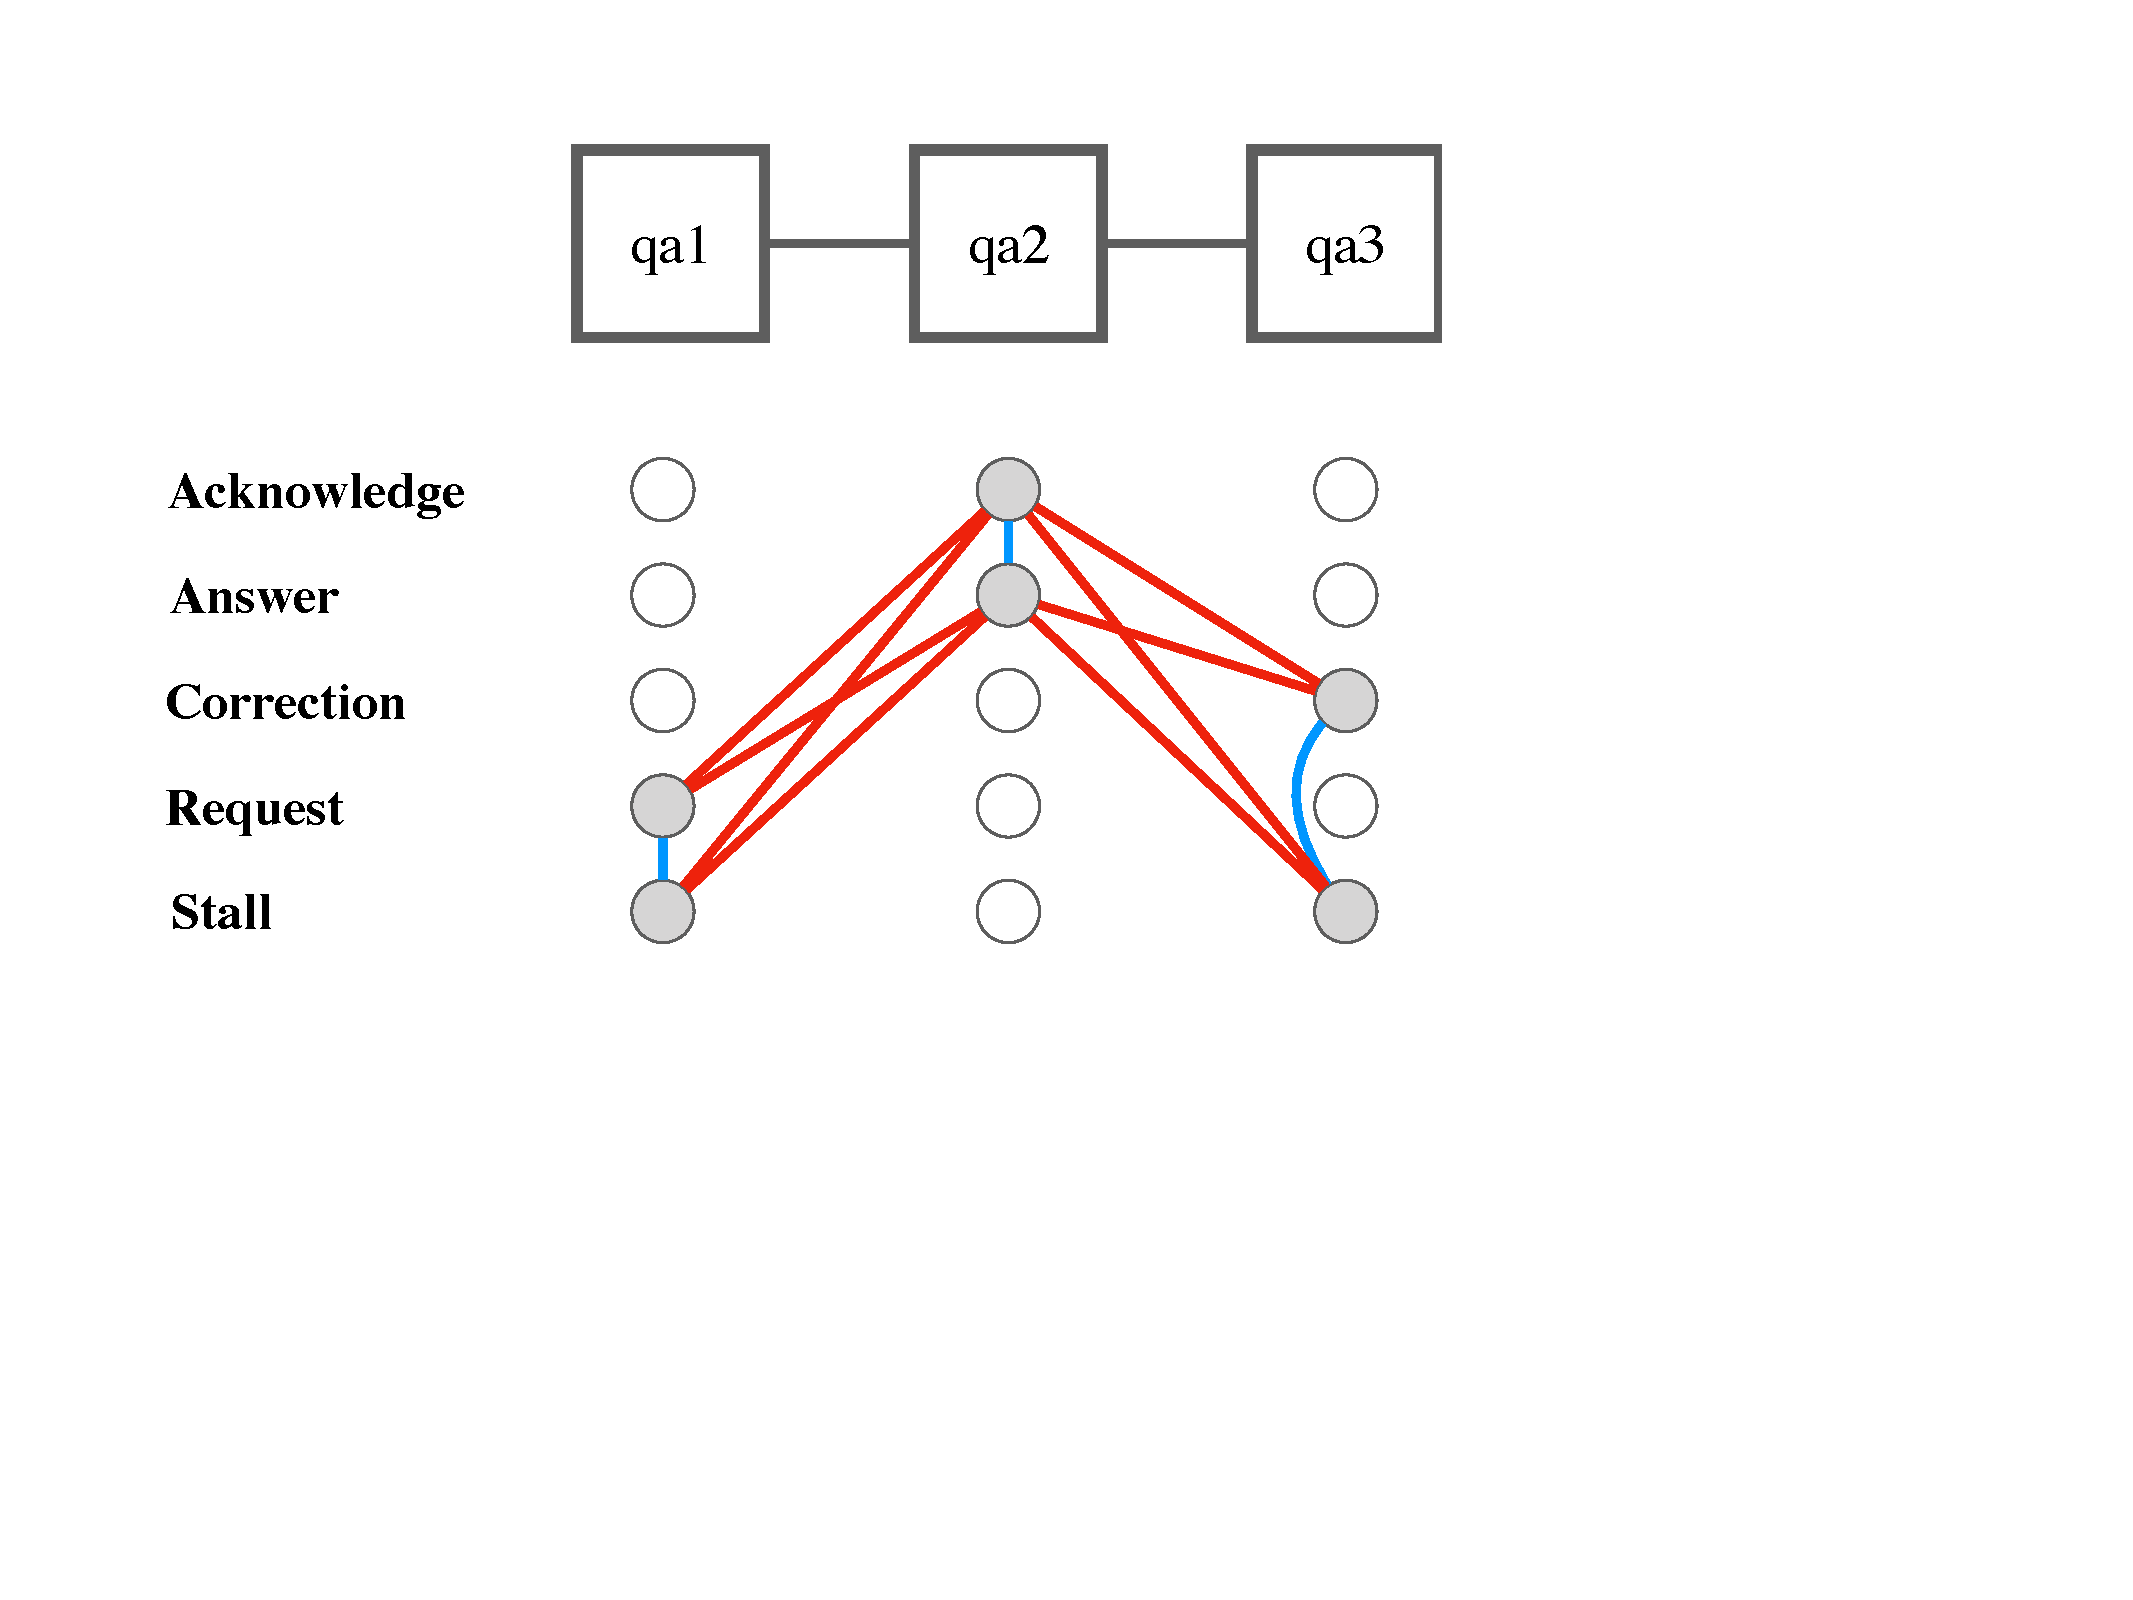
\includegraphics[width=1\linewidth]{plots/multilabel_context.pdf}
  \captionof{figure}{\textsc{Multi-label+context}: predict the set of dialog acts for a question-answer pair and history of question-answer pairs, while modeling correlations within a set (blue) and across time steps (red).}
  \label{fig:multilabel_context}
\end{minipage}
\end{figure}

\noindent {\bf Model 1: \textsc{Multi-label}.} My first task is \emph{multi-label classification}: given a question-answer pair, predict the gold set of labels (Figure \ref{fig:multilabel}). This task is often applied to classifying longer documents (news articles) that are tagged with multiple keywords. Importantly, in this setting (and expectedly in my data as well) the labels are often correlated; for example, a document labeled as \textit{basketball} is likely to also be labelled as \textit{sports}. I propose to explore two models that account for this correlation: Classifier Chains (\textsc{CC}) \cite{Read:2011} and structured prediction of sets \cite{Rabinovich:2017}. \textsc{CC} transforms the problem into a \emph{chain} of binary classification tasks. This approach offers considerable flexibility because any binary classifier can be used, such as SVM or Naive Bayes, but the predictions are made sequentially. Structured set prediction, on the other hand, models features jointly and restricts the predicted set to be connected in a graph. This model uses structured max-margin during learning and set-F1 as the loss function (to reflect order invariance).

For evaluation, there are two groups of standard metrics that focus either on evaluating the predictions on an example-by-example basis (\emph{example-based}) or on a label-by-label basis (\emph{label-based}). The \emph{label-based} Hamming loss evaluates the fraction of labels that are predicted incorrectly (lower is better). The \emph{example-based} precision, recall and micro-F1 are averaged by the weight of each label. 

\noindent {\bf Model 2: \textsc{Multi-label+context}.} While the previous models account for correlations of labels within a set, they do not consider the surrounding context. Knowing the labels of the previous question-answer pairs is helpful in predicting the current question-answer pair. In the Zuckerberg example in Table \ref{tab:example}, the first question-answer pair label set includes \texttt{request for information}, which naturally predicts \texttt{answer} in the following question-answer pair. I thus reframe the task as follows: given a question-answer pair and the context of past question-answer pairs with their predicted labels, predict the gold set of labels (Figure \ref{fig:multilabel_context}).  Interestingly, there is little work in NLP on predicting \emph{sequences} of multiple labels (though not surprising since most multi-label applications are document classification tasks). The most straightforward approach to account for context is to augment the \textsc{Multi-label} model with features extracted from the question-pair history. 

An alternative modeling solution is to view the task as an extension of the \emph{sequence labeling} problem, where the model predicts multiple instead of single labels. The standard task of (single-label) dialog-act classification is typically framed as a sequence labeling problem. For example, \citet{Joty:2018} employ a neural-CRF to capture these dependencies for speech acts in asynchronous conversations. I can use a similar CRF model which captures short-distance dependencies and then use Integer Linear Programming to enforce hard constraints (loopy belief propagation yields probabilistic constraints but may prove unnecessarily complex). 

% I intend to investigate the SVM proposed in \citet{Li:2010} which learns a joint kernel to model both types of dependencies. This model is applied to the task of predicting the set of concept tags assigned to a given video shot in a sequence of video shots. 

For evaluation, I use the standard multi-label metrics of Hamming loss and precision, recall, micro-F1.

\begin{figure}
\centering
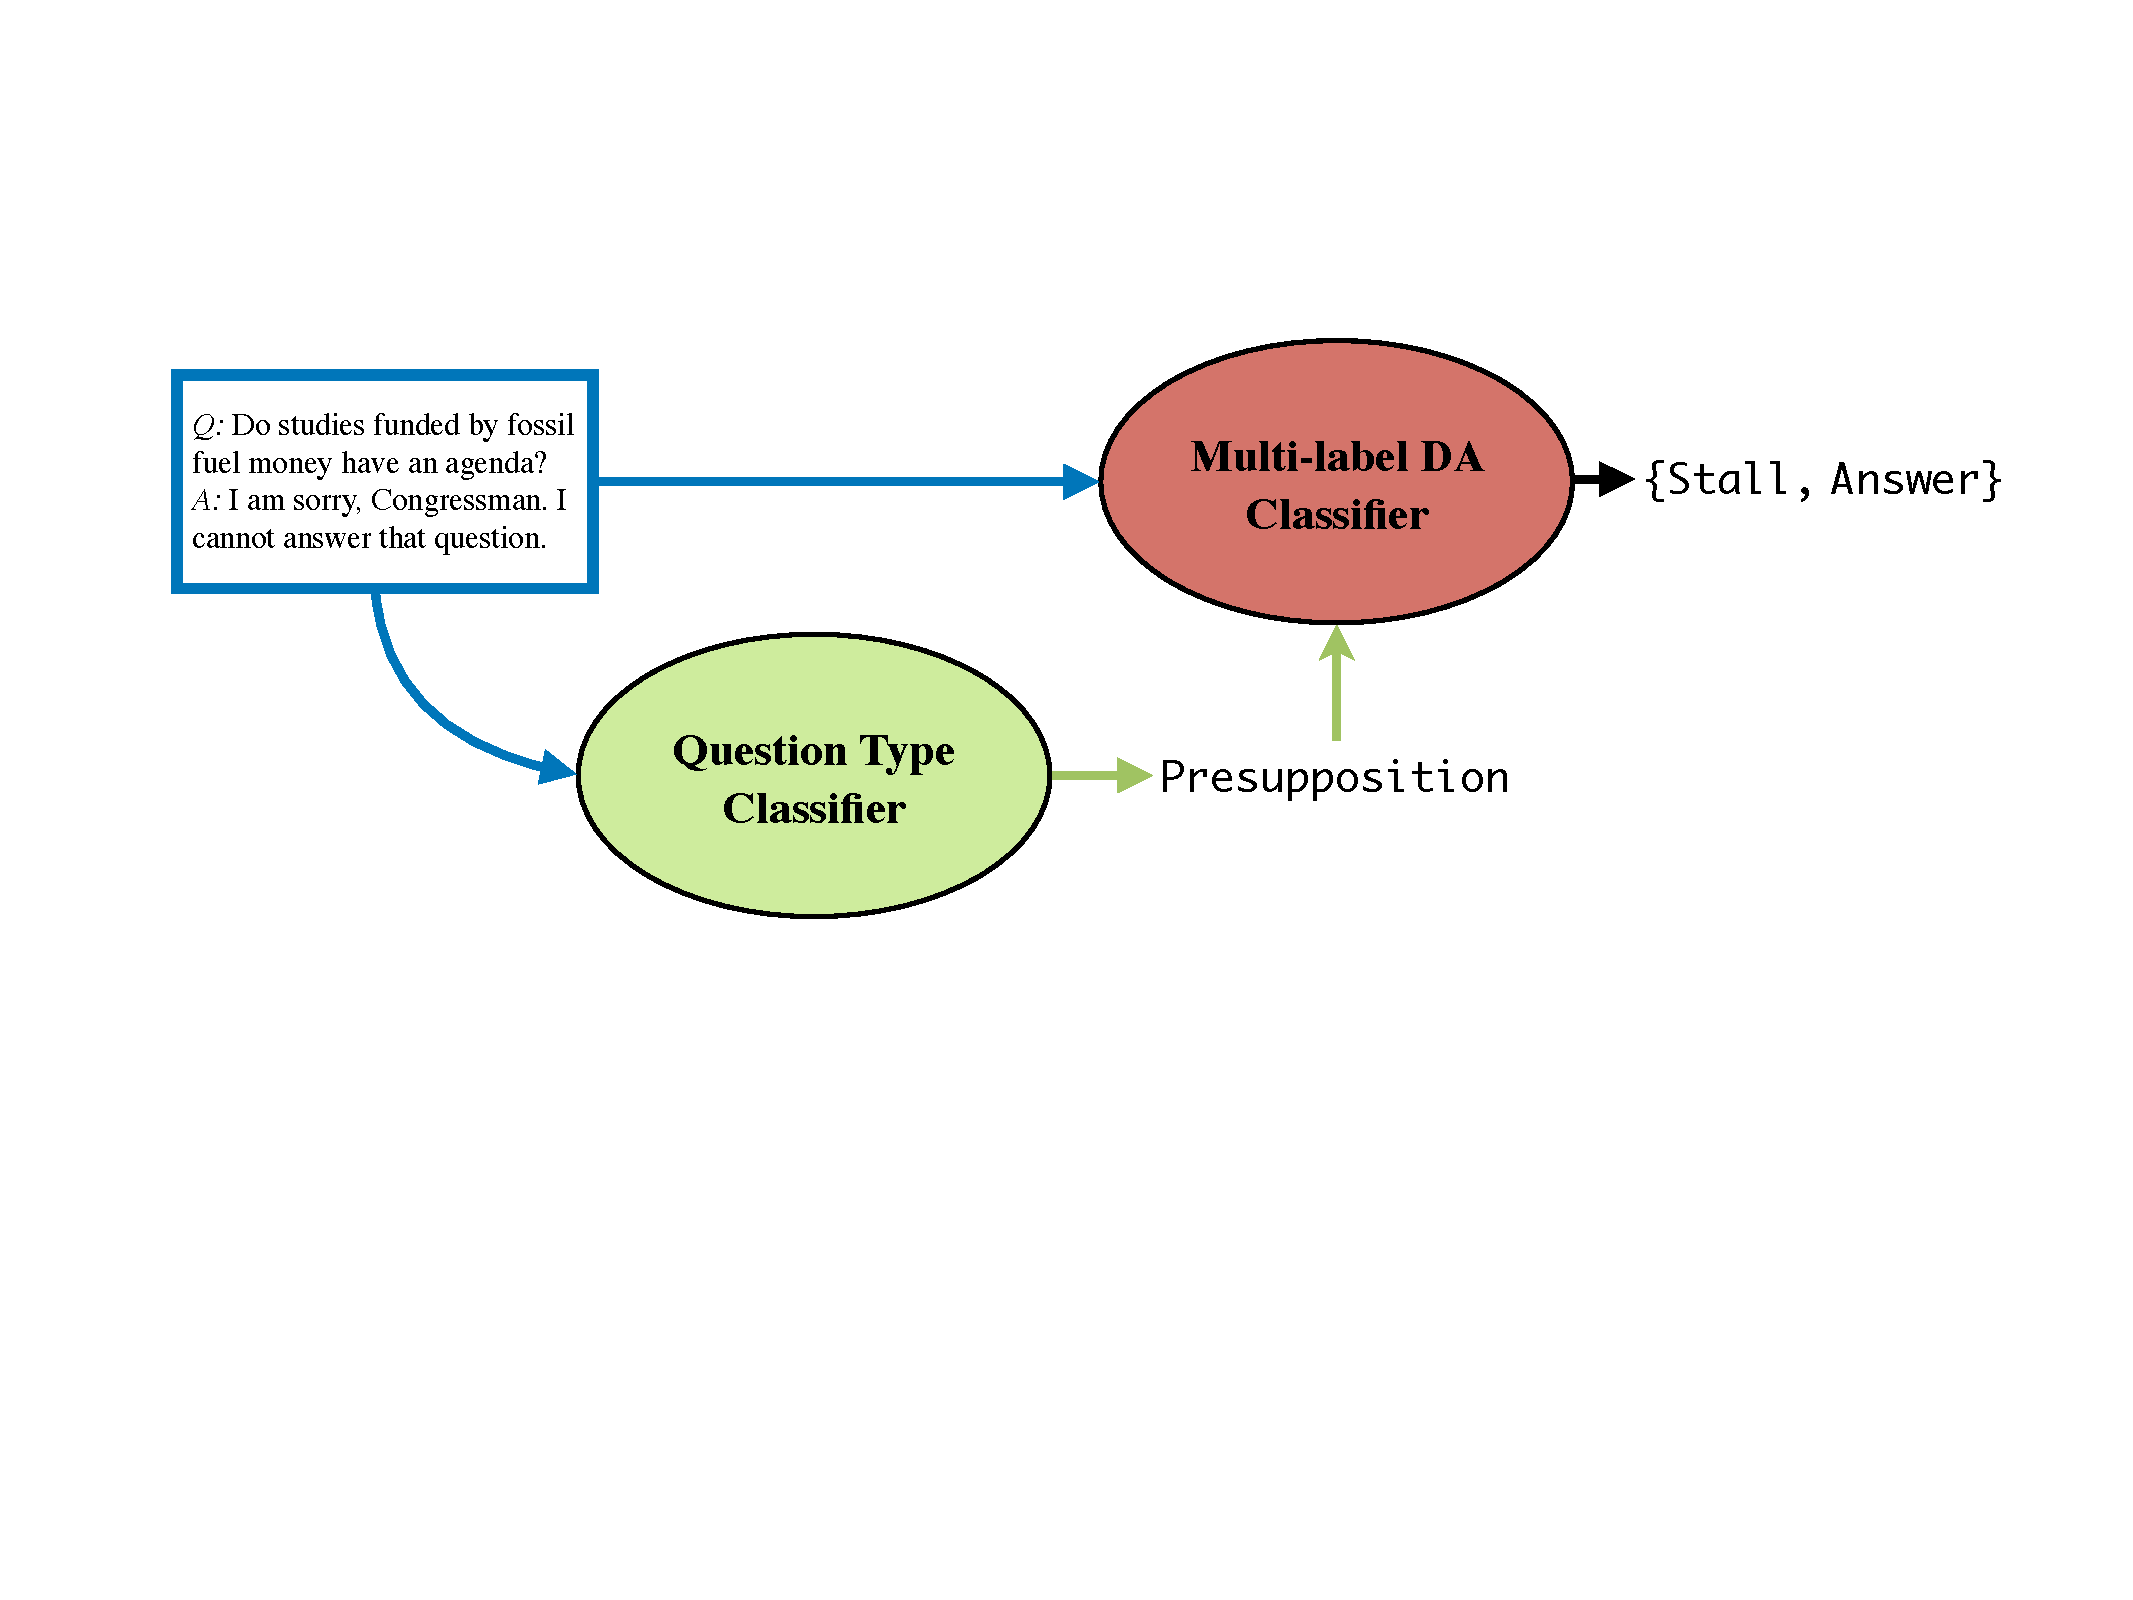
\includegraphics[width=\columnwidth]{plots/multilabel_question.pdf}
\caption{\textsc{Multi-label+question}: A preprocessing step classifies the question type; this label along with the question-answer pair are fed to the multi-label classifier.}
\label{fig:multilabel_question}
\vspace{-1em}
\end{figure}

\noindent {\bf Model 3: \textsc{Multi-label+question}.} Within a question-answer pair, the nature of the question can help inform the labels. As noted earlier, ``loaded'' questions often lead to indirect answers. I propose a preprocessing step to classify the question type, and then feed this prediction into the multi-label classifier (Figure \ref{fig:multilabel_question}). While I could also learn these two tasks jointly in a multi-task setting, prior work shows this configuration is most helpful when the auxiliary task data is considerably larger \citet{Luong:2015}, which is not the case here. 

For the preprocessing single-label classification task, I evaluate with accuracy and precision, recall, F1. For the main multi-label dialog act classification task, I evaluate with Hamming loss and precision, recall, micro-F1. 


\section{Long Term} 
The long-term experiments focus on capturing the subjectivity of discourse by modeling particular annotators, and finally returning to the notion of conversations as games by tracking the winners across turns in a conversation.

\subsection{Crowd-sourcing Phase 2.}
\label{subsec:phase2}
In the second phase of crowd-sourcing, I use a similar setup as in Phase 1, but instead ask the annotator to choose the \emph{single} best dialog act for a question-answer. Additionally, I ask the annotator to choose the ``winner'' of that turn. Unlike in a debate setting, deciding who has won in a question-answer setting is not intuitive or clearly defined. The Congressional hearings are nevertheless combative, and I could reframe the task to deciding who has the upper hand. 

\subsection{Experiment 2: Subjective discourse} The ultimate task is to determine how a person will interpret a discourse, given their biases. However, capturing biases is a  challenging task that significantly deviates from the core focus of this dissertation to show that discourse is ambiguous. Instead, I argue that we can inherently capture the bias of a given annotator by making predictions for that specific annotator. In particular, given a question-answer with the annotator id and history of labeled question-answers, the model must predict the label chosen by that annotator. This experiment, however, relies on having enough labels from one single annotator, which may not be feasible, and instead annotators may need to be clustered together based on some measure of labeling similarity.

\begin{figure}
\centering
\begin{subfigure}{.47\textwidth}
  \centering
  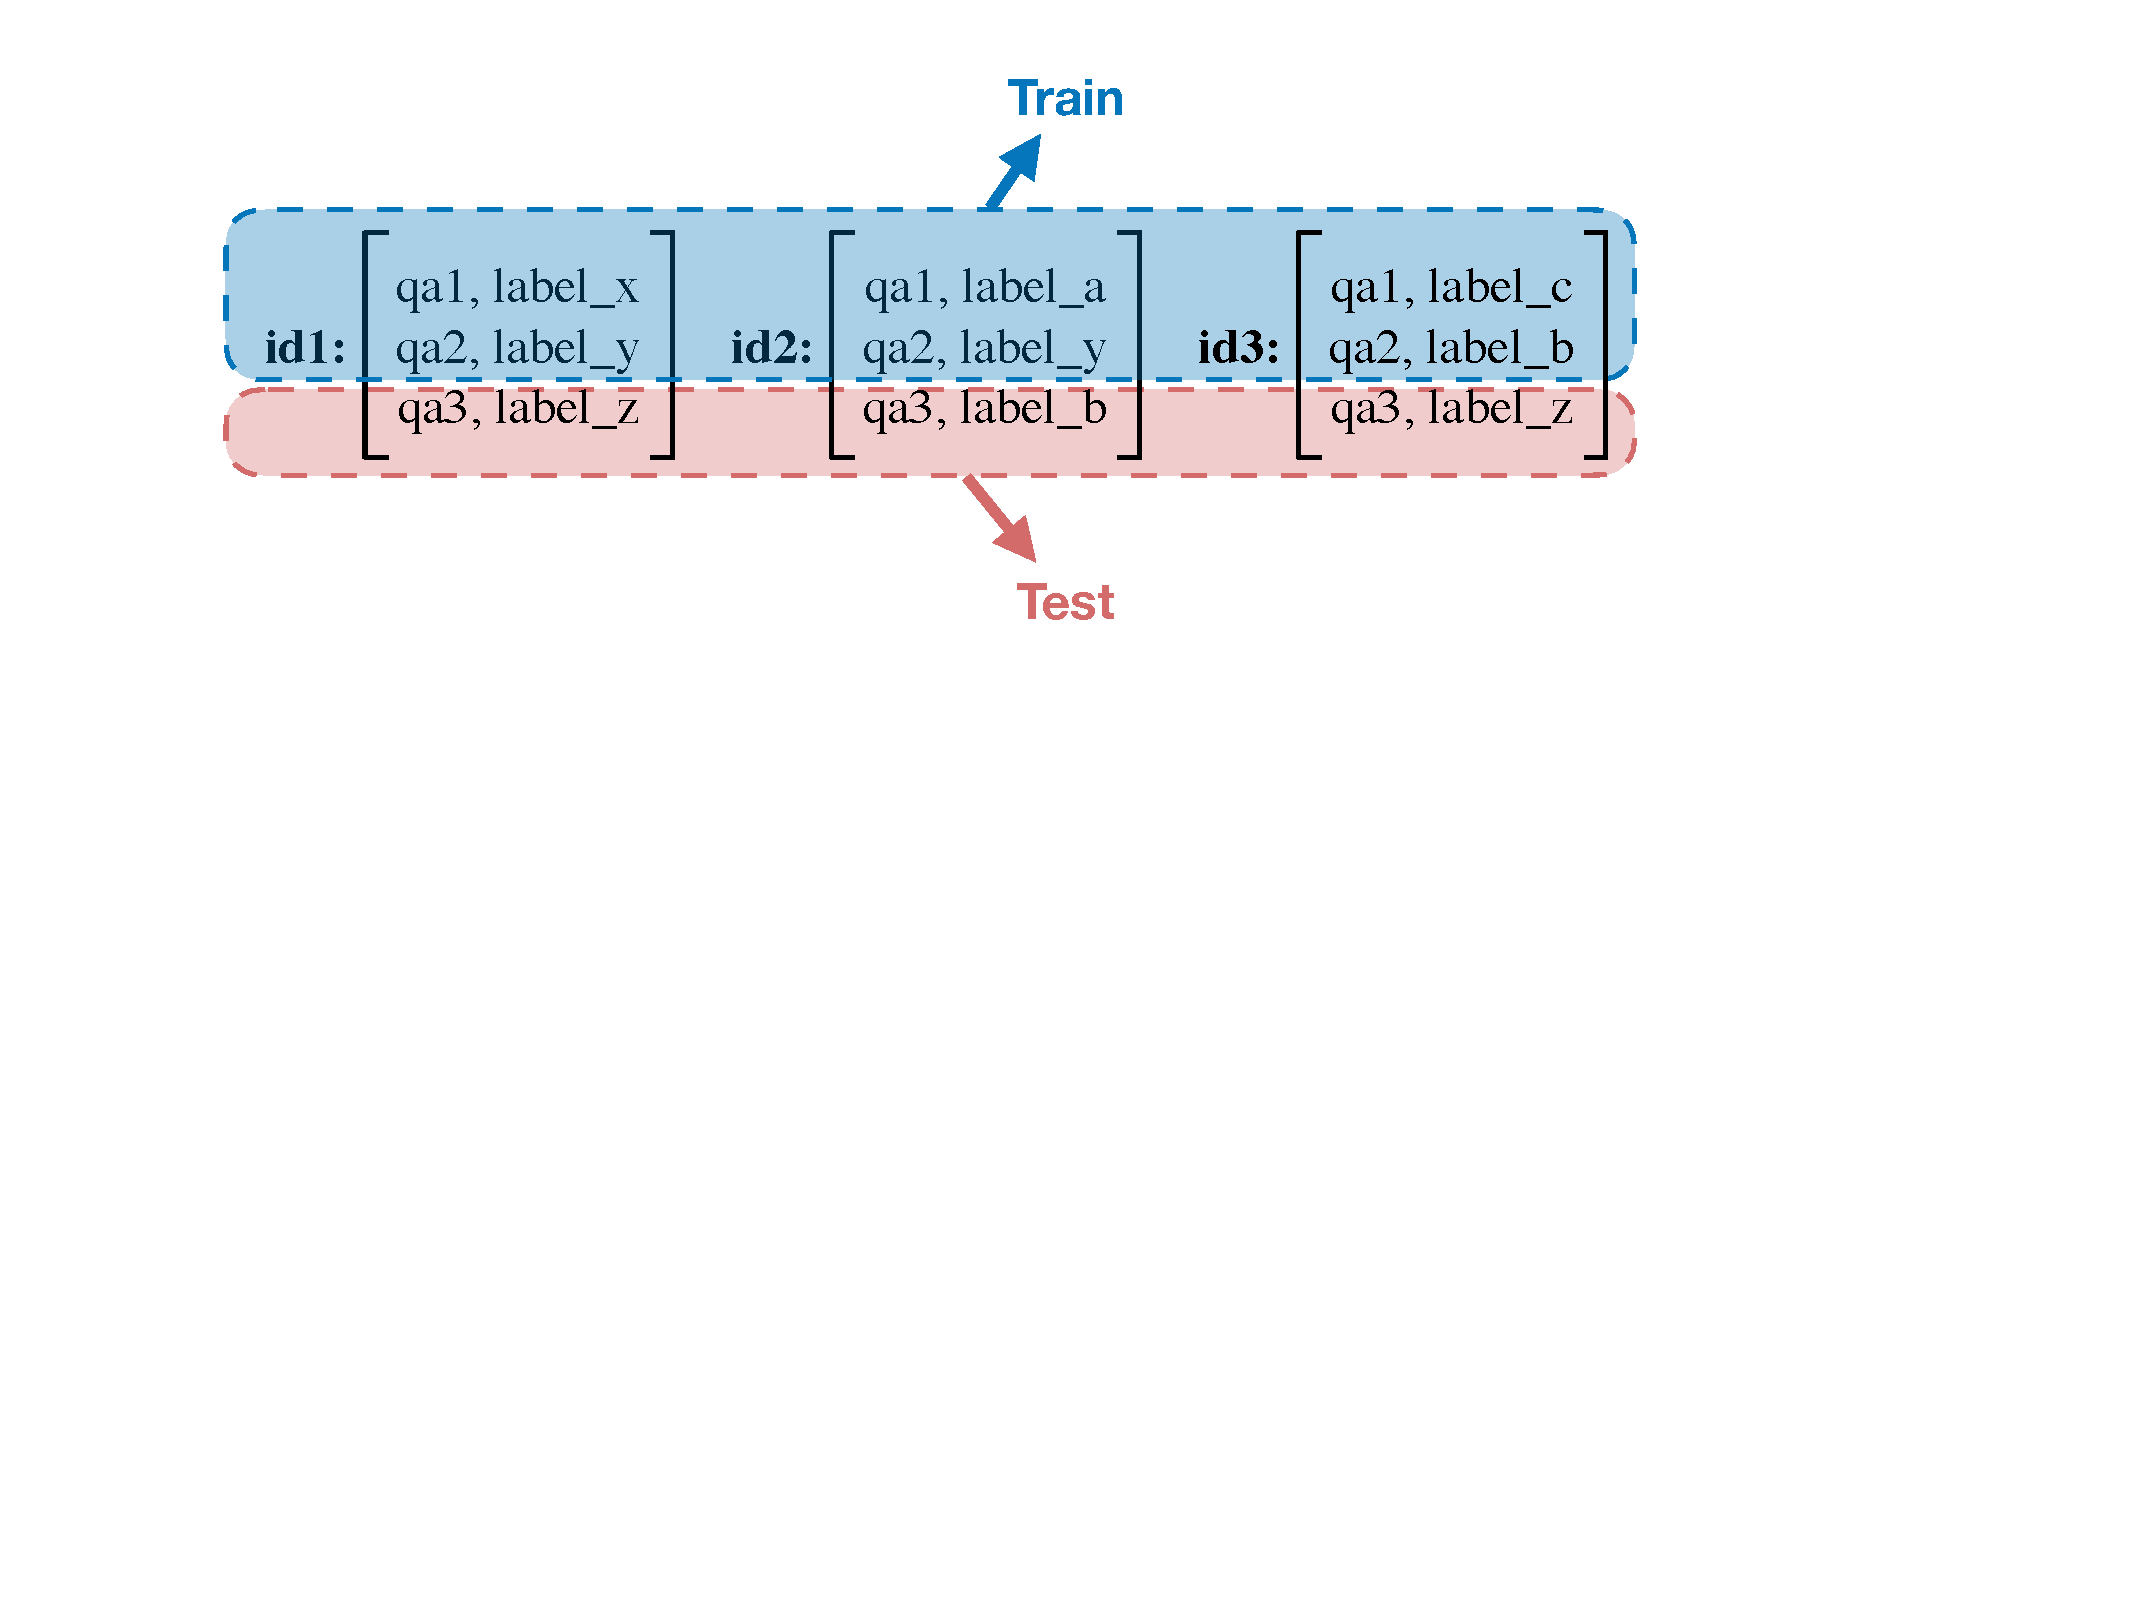
\includegraphics[width=1\linewidth]{plots/anno_known.pdf}
  \caption{Seen annotator}
  \label{fig:split_seen}
\end{subfigure}%
\hfill
\begin{subfigure}{.47\textwidth}
  \centering
  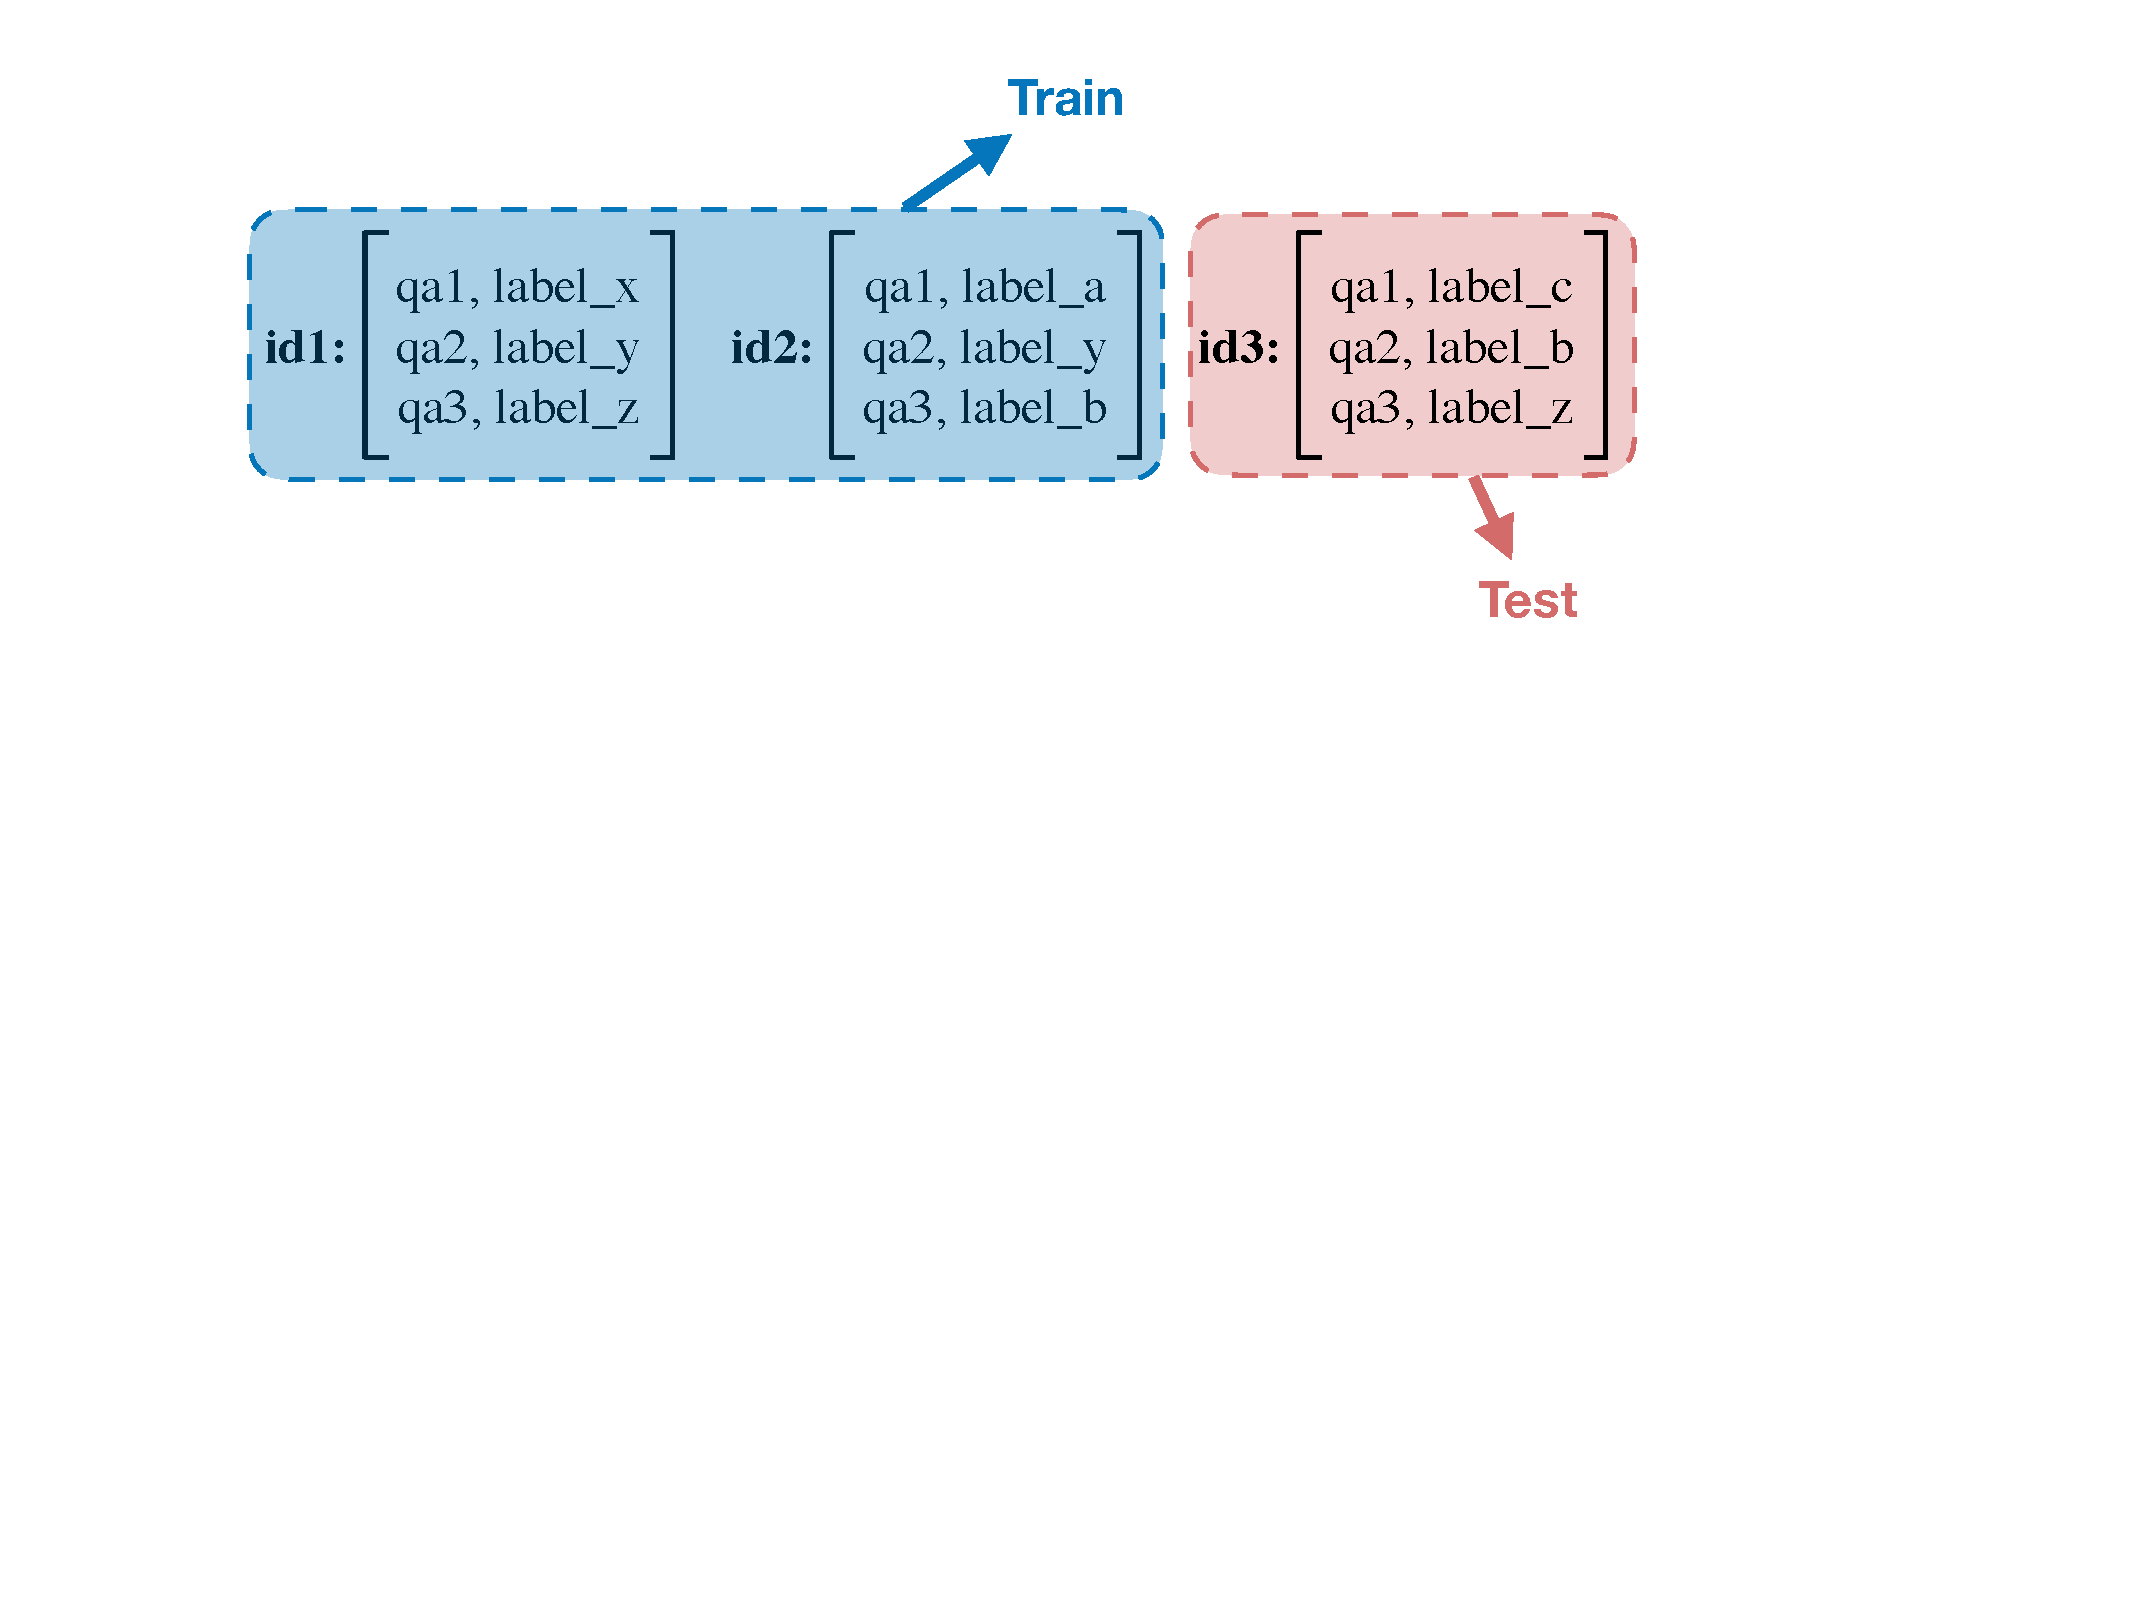
\includegraphics[width=1\linewidth]{plots/anno_unknown.pdf}
  \caption{Unseen annotator}
  \label{fig:split_unseen}
\end{subfigure}
\caption{Data splits for modeling a seen annotator (left) or an unseen annotator (right) at test time.}
\label{fig:splits}
\end{figure}

\noindent {\bf Model 1: Seen annotator.} This model trains on all annotators, but part of their annotations are held out (Figure \ref{fig:split_seen}). At test time, the model predicts the label for a question-answer, given a \emph{seen} annotator id with their history of labelled question-answers . This task can be addressed with standard single-label classifiers.

\noindent {\bf Model 2: Unseen annotator.} This model trains on all annotations, but a portion of the annotators are held out (Figure \ref{fig:split_unseen}). At test time, the model predicts the label for a question-answer, given an \emph{unseen} annotator with their history of labelled question-answers. Taking into account annotator biases is similar to the task of persona-based dialogue generation. In this setting, the model predicts the next utterance in a dialogue conditioned on some representation of the speaker. Here, the speaker is not a specific user, but a more general persona meant to encompass a group of people. \citet{Zhang:2018} create artificial profiles for different personas and elicit dialogues from crowd-sourced workers that adopt these personas. They find that conditioning on the persona yields utterances that are likelier as measured by perplexity (although human judgements of consistency do not show significant differences). Because I do not have explicit information on the annotators as in \citet{Zhang:2018}, I plan to explore the approach in \citet{Li:2016} that learns an embedding for the speaker.

\subsection{Experiment 3: Tracking conversation winners} 
The prior experiments focus on capturing the ambiguity and subjectivity of discourse, by being able to predict multiple ground truths and a single ground truth for a particular annotator. These experiments lay the groundwork for the final goal of tracking conversation winners. Returning to the conversations-as-games theory in \citet{Asher:2018}, the third-party reader makes judgements at each turn in the conversation of who the winner is, and finally who the overall winner is. 

Deciding on a final winner is reasonably straightforward in debate-like scenarios. For example, \citet{Zhang:2016} create a model to predict the winner of Oxford-style debates (in particular, two-sided debates on the NPR show ``Intelligence Squared''). Audience members are polled at the beginning of the show to vote for one side, and then again at the end. The ground-truth winner is determined by the speaker who is able to flip the most votes. While this only provides a signal at the end, the data also includes audience feedback (such as laughter and clapping), which \citet{Potash:2017} uses as a signal for the winner of a particular turn in an RNN that models each time step.  
The goal of this experiment is to predict the winner across a sequence of conversation turns, given the annotator and their labeled question-answers.

\section{Chapter Summary}
In my proposed work, I aim to capture the ambiguity and subjectivity of discourse. I propose a new dataset that has multiple judgements for a single data point to reflect the inherent ambiguity in some relations, as well as judgements across entire conversations to model the bias of particular annotators. I propose a series of experiments that model these properties of discourse and finally putting these pieces together to understand a conversation as a game being judged by the biased annotator.  